\chapter{Scene Recognition}
In this chapter, we discuss the process of how a scene is recognized by detected events in the testing clip. 
This chapter includes the issue of mining scene-event relations from downloaded script data.
Then a segmenter algorithm is used to segment audio data for event detection. 
In the last, the detected event sequence is used for scene recognition. 

\section{Scene-Event Relation Mining}
\subsection{Event Expanding}
In the eventlist we created, the events are all in their original form. 
However, in the movie, play or TV series data, the words are used to describe real world events. 
They inevitably have different forms, like plural of nouns, and various tenses for verbs. 
In order to match these diverse cases, we expand the words in our eventlist to their possible forms to accomdate the reality. 

The idea of event expanding is that we find the plural forms for nouns, and find different verb tenses. 
Then if we are going to match for some events, we not only match its original form, but also other forms. 
We use the Nodebox English Linguistics library\footnote{https://www.nodebox.net/code/index.php/Linguistics} to complete this expanding task. 
It provides some convinient tools for nouns pluralization and verb conjugation, i.e., create derived forms of a verb from its principal form. 

\subsection{TF-IDF Calculation}
As mentioned before, the goal of our project is to build a relation between audio scenes and audible events and then infer scenes by this relation.  
We have already introduced the data we are going to use: scripts for movie, play, TV series, etc. 
In the chapter of data preparation, we have splitted out the small contexts in scripts. 
Each context has one scene attributed to them, and in this section, we are going to explore the analysis of contexts under the condition that its scene is known. 

The mathematical simplification here is to calculate the posterior probability of $P(S|E)$, assumming $S$ is a scene, $E$ is an audible event. 
Using this probability, we could basically tell what scene is the most likely one if we have detected the presence of event $E$. 
Term frequency of each event in respective scenes give us a perspective into this issue. 
It is natural to think that a scene is recogized if a high-frequency event in its context is detected. 
However, mearly using this term frequency may not work out in the case of common events. 
Common events are the audible events that appear in lots of scenes, so their presence do not provide a discernible knowledge for what is the most likely scene. 
In order to calculate how important a audible event is in identifing a scene, we need a metric for calculating event distinctiveness. 
To tackle this issue, Term Frequency-Inverse Document Frequency (TF-IDF) statistic is used for calculating event distinctiveness. 

The original TF-IDF statistic is used to reflect how important a word is to a document in a corpus. 
In a corpus with many documents, the TF-IDF value of a word to one document increases propotionally to the frequency of that word in that document. 
But the value decreases if the word appears in many other documents. 
Overall it measures the distictivenesss of word-document pair. 
We use the idea of TF-IDF statistic, but applied to our special case. 
In our case, the corpus refers to all of the context files, each contains one scene. 
Document is therefore one scene type. 
Word here means an audible event. 
Suppose $e$ and $s$ represent a event and a scene, respectively. 
$f(e,s)$ denotes the number of context that e has appeared in it among all the contexts that belong to scene $s$.  
$N$ is the total document number in consideration, and $N_e$ is the number of documents the event $e$ appears in. 
Hence TF and IDF are calculated as: 
\begin{equation}
\begin{split}
 TF &= \log{1+f(e,s)} \\ 
 IDF &= 1 + \log{\frac{N}{N_e}}
\end{split}
\end{equation} 

After these two values are calculated, the TF-IDF value are therefore get by multiplying them together. 
\begin{equation}
 \text{TF-IDF} = TF \times IDF 
\end{equation}

In the evaluation part, we would perform an experiment on 10 scene classification problem. 
The 10 audio scenes are: \textit{bathroom, beach, concert, forest, kitchen, office, park, restaurant, street}, and \textit{subway station}. 
Table \ref{table:exampleMap} shows the top 10 events ranked by TF-IDF scores for these 10 scenes. 
Note that in scene ``concert'', there is only 7 events listed there due to the limited data on this scene. 
This scene-event map with their TF-IDF scores could be viewed online\footnote{\url{http://adapt.seiee.sjtu.edu.cn/~xunxu/asr/map.txt}}. 

\begin{table}[htb!]
\centering
\resizebox{\textwidth}{!}{
\begin{tabular}{ll}
\toprule
Scene     & Top 10 events ranked by TF-IDf\\
\bottomrule
bathroom & running+water, toilet, faucet, toothbrush, shower, drawer, drain, talk, paper, bowl \\ 
beach & seagull, sand, boat, talk, wave, sea, car, laughter, drink, wood, running \\ 
concert & piano, applause, crowd, chorus, child, cry, talk \\ 
forest & tree, wood, dirt, talk, running, bird, river, car, leaf, grass, wind\\ 
kitchen & drawer, cutlery, microwave, dish, kettle, talk, bowl, phone, toaster, running+water\\ 
office & desk, drawer, page+turn, talk, phone, printer, paper, chair, leaf, typewriter\\
park & talk, car, tree, laughter, dog, child, grass, crowd, running, phone\\ 
restaurant & talk, drink, laughter, phone, car, leaf, paper, dish, ring, chair, write \\ 
street & car, truck, subway, talk, traffic, engine, siren, phone, running, laughter \\ 
subway station & subway, train, car, tube, talk, pace, crowd, metal, phone, vehicle \\ 
\bottomrule
\end{tabular}
}
\caption{An example of scene-event map}
\label{table:exampleMap}
\end{table}

% concert don't have much contexts


\section{Audio Segmentation}
Once the models are built, we are ready to use it to test on a potential event clip. 
But for the problem of scene recogniton, the testing data are a clip which may contain multiple events. 
We apply a segmenter to split out the silence or background noise part, and return segments containing some events to be detected. 

There are lots of research carried out on the segmentation of audios.
Some may simply use the average frame energy as the threshold to cut the clips, while other complicated methods involve more features and even use machine learning techniques. 
In this project, we use a method of setting a threshold combining frame energy and spectral centroids, and this method is described in \cite{giannakopoulos2009method}.
This method uses two features from audio:
\begin{itemize}
\item{Frame Energy: this features depicts the overall energy level of one frame. 
Typically frames where there are some events happening have a higher energy than silent frames.
Let $x_i$ be the signal value of the $i$-th frame, and suppose there is N data points in this frame. 
Then frame energy $E_i$ of the $i$-th frame is calculated as:  
\begin{equation}
E_i = \frac{\sum\limits_{n=1}^N(x_i(n))}{N}
\end{equation}
}
\item{Spectral centroid: this represents the "center of gravity" of the audio spectrum. For example, the spectral centroid of the $i$-th frame (denoted by $ C_i$) is given by the equation:
\begin{equation}
C_i = \frac{\sum\limits_{k=1}^Nk\times Amp(k)}{\sum\limits_{k=1}^NAmp(k)}
\end{equation}
In this equation, $Amp(k)$ is the amplitude corresponding to bin $k$ in Discrete Fourier Transform (DFT) spectrum. 
So a higher spectral centroid denotes a higher frequency in this frame. Because noises are often in a low frequency, we could use this feature to filter them out. 
}
\end{itemize}

After these two features are calculated for every frames, they are further smoothed and averaged to get a threshold. 

% A segmentation example 
\begin{figure}[htb]
\centering
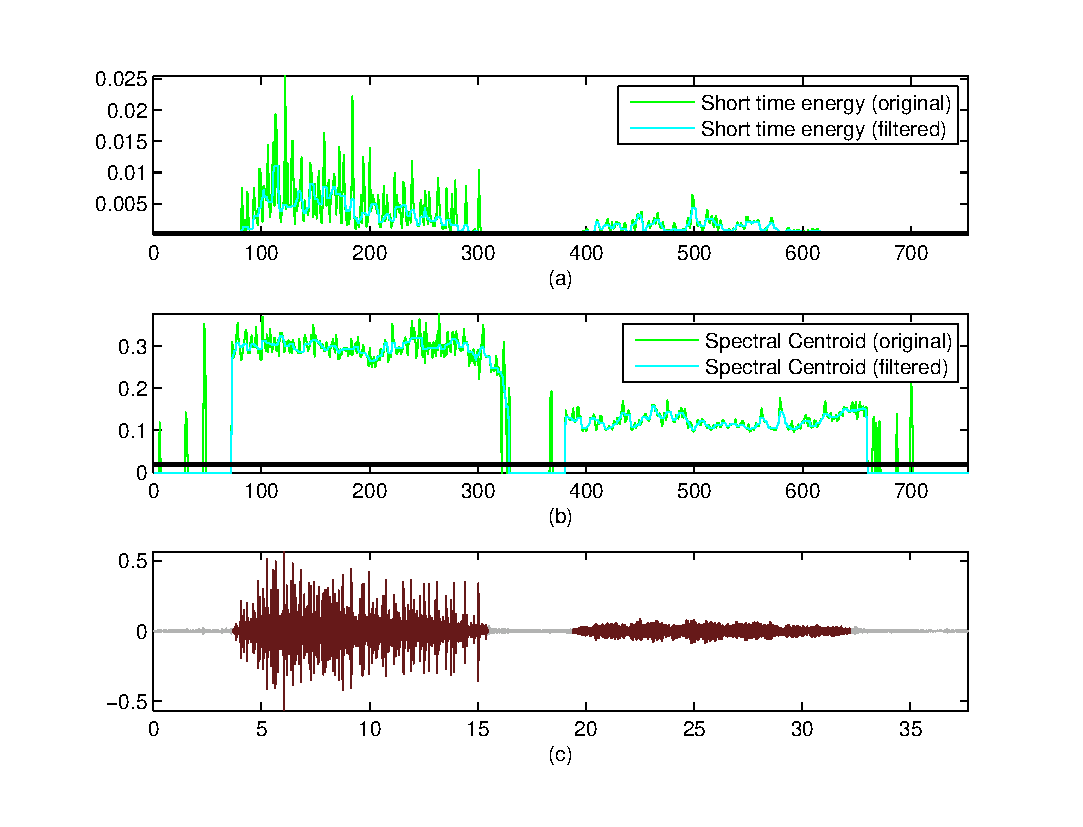
\includegraphics[scale=0.8]{figure/scenerecog/segment}
\caption{A segmentation example}
\label{fig:segment}
\end{figure}

Figure \ref{fig:segment} is a example of segmenting an audio clips using the segmenter. 
The original audio is recorded in a concert containing two audible events, the first half part represents the sound of applausing, and the latter half part represents the sound of instrument tuning. 
In this figure, subfigure (a) and (b) are audio features of short time energy and spectral centroid respectively.  
In these two subfigures, the green line is the original feature data, and the cyan line is the filtered verson of feature data. 
In the segmenter, median filter\footnote{\url{http://cn.mathworks.com/help/signal/ref/medfilt1.html}} is applied in the feature sequence using 5 windows, each window is a frame of 50 milliseconds. 
After filtering, we could see that first the short time energy for \textit{instrument tuning} is very low, nearly reaching the threshold (represented by the thick black line). 
At the same time, \textit{instrument tuning} has a relative higher spectral centroid with regard to the threshold in spectral centroid. 
For the \textit{applause} sound, the two features for it are both above the corresponding threshold.  
In the end, we could see in subfigure (c), there is two segments highlighted by a dard red area. 
These two segments are cut out for event detection. 

\section{Scene Inference}
Once a event sequence is detected, we use that sequence of events to infer the scene we think it's the most likely one. 
Suppose $S$ denotes a scene, $E_i$ represents the $i$-th detected event, and $i$ ranges from $1$ to $n$. 
Hence the problem of finding the most likely scene for a detected event sequency could be mathematically shown as: 
\begin{equation}
S^* = \operatorname*{arg\,max}_{S} P(S|E_1,E_2,...,E_n)
\end{equation} 

$S^*$ here we get would be the most likely scene from the observation of $E_i, i = 1,...n$.  
Yet, in order to calculate this posterior probability, we assume events are independent. 
This assumption may seems strict because some events are more likely to occur together in one scene. 
For example, in concert, we may hear \textit{applause} follows some \textit{piano} performance. 
But we think treating audible events independently could get reasonable result if the events are correctly detected by itself. 
So currently we sticks to the independence assumption. 
Under this assumption, we can rewrite the posterior probability as: 
\begin{equation}
P(S|E_1,E_2,...,E_n) = P(S|E_1) \times P(S|E_2) \times ... \times P(S|E_n)
\end{equation}

Sometimes, one segment may contain multiple events overlapping together. 
So in this case, only using the top 1 detected events is not enough. 
So we use the top 3 detected events for each segment, and their posteriors are used as weight. 
After multipling with the TF-IDF scores of each event to each scene, we could get a score for every scene. 
Then the highest scored scene are choosen as the recognized scene. 

\section{Summary}
The process of scene recognition is reviewed here. 
Because our system works in a way of first detecting events out of a scene clip, we apply a segmenter to segment out the silence part of a scene clip. 
Then a previously mentioned event detection model is used to detect events from the segments. 
After detection, we could get a detected events sequence. 
The process for scene recognition is conducted with the help of a score we calculated from script data. 
The score is the Term Frequency-Inverse Document Frequency (TF-IDF) of a event to a scene. 
The idea of this score is similar to its original application in identifying important words for a document. 
In our problem, we use it to identify important audible events for a scene. 
We use this TF-IDF value as the weight for event in contributing a scene. 
After all the calculation, the scene which enjoys a highest score is outputed as the detected scene. 
